\chapter{The physical Track}
Author: Florian Schwarzl

Being able to drive along a simulation of the track is only a partial success. In order to prove successful, the trained algorithm is required to complete multiple runs on a real track using our DeepRacer vehicle. When training an autonomous vehicle with reinforcement learning for a real-world scenario, it is logical to create the simulation so that is represents the real environment as precisely as possible. However, since this is a leaning environment and the environment is set by Amazon, we are required to achieve the exact opposite. Effective testing requires the creation of a real-world track that fits those from the training simulation. How accurately the physical course represents the simulated one will have a direct impact on the performance of the vehicle.

\section{Track Layout}
A total of 34 simulation worlds are provided. The real track is modelled after the standard oval track. It is a simple loop with no additional curves. Which track to choose is impacted primarily by the space available. Since the real track should resemble the simulated environment as closely as possible, choosing a track which can be built and placed in its entirety is important. Otherwise the trained models might perform poorly, although a robust model will still be able to traverse a track that is not an exact replica of the learned environment. 
\begin{figure}
    \centering
    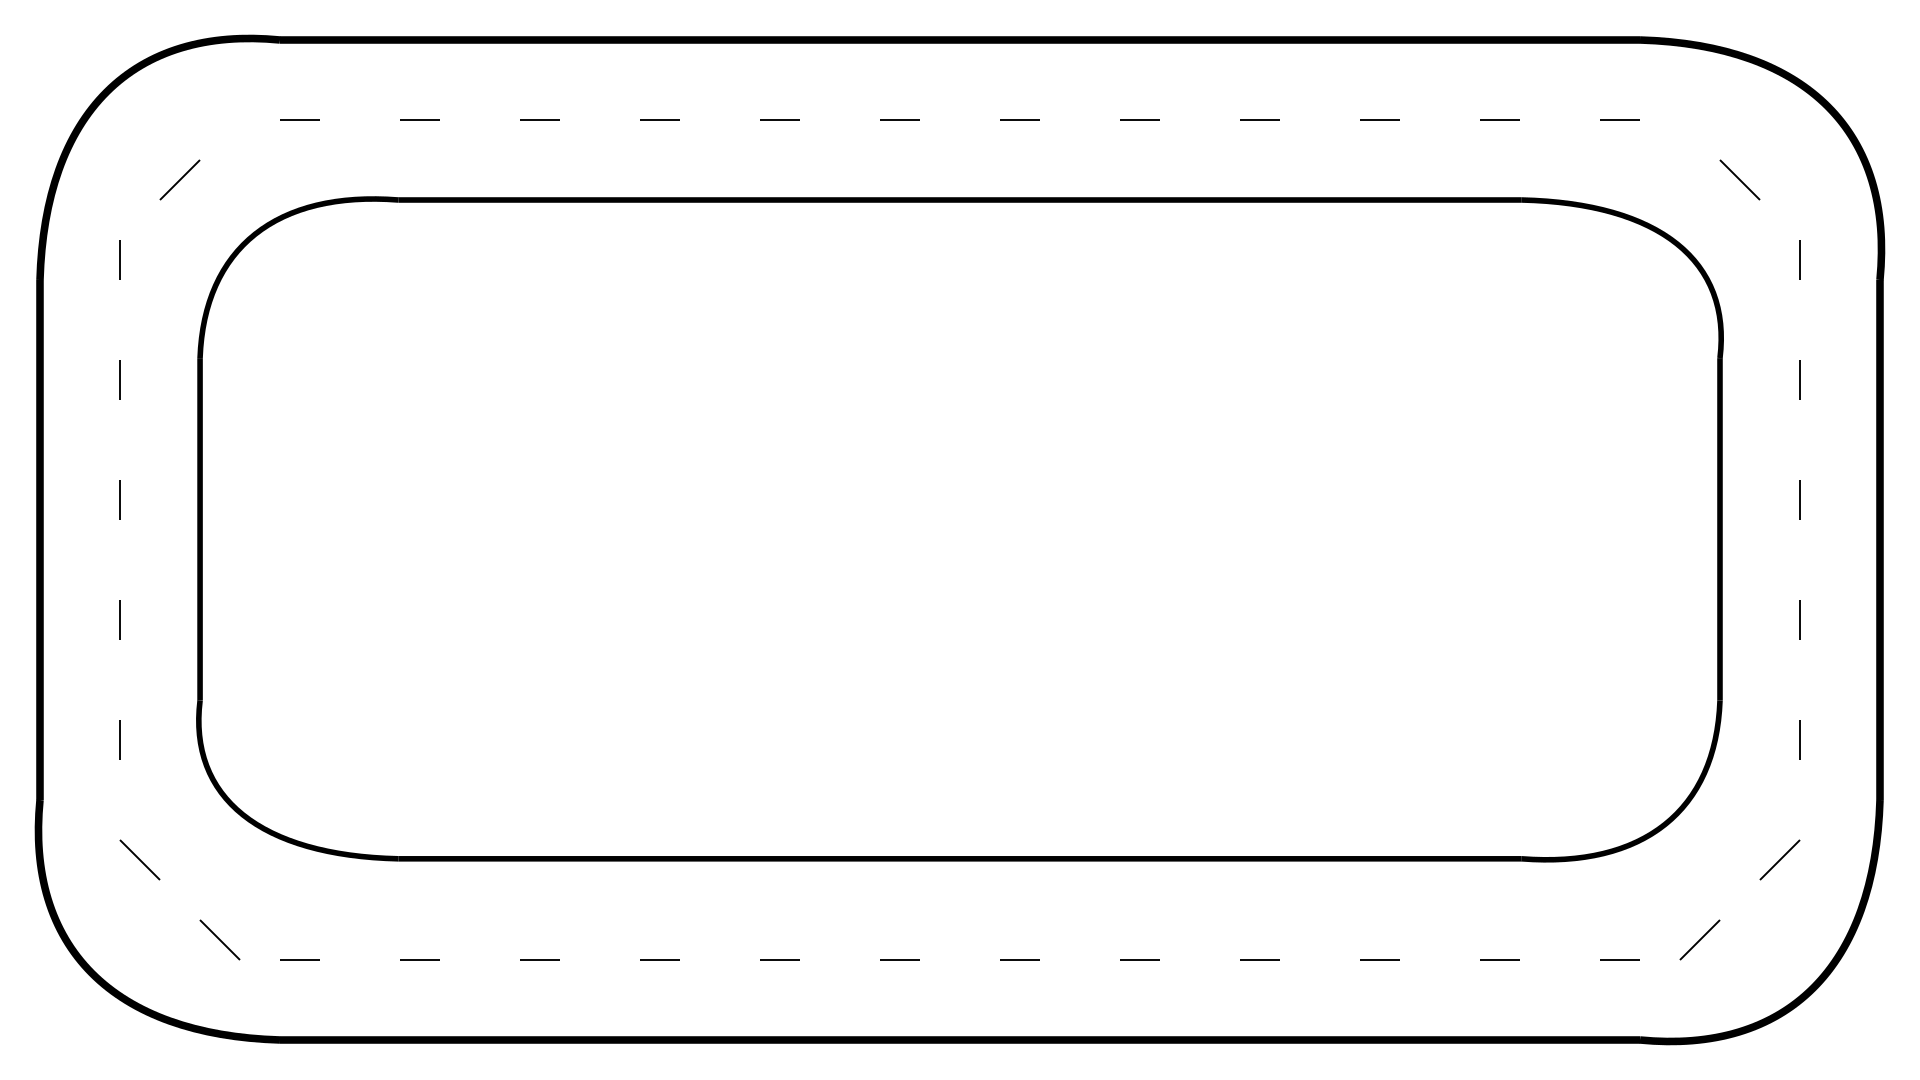
\includegraphics[width=.85\textwidth]{images/oval_track.png}
    \caption{Oval track layout}
    \label{fig:track}
\end{figure}

The initial decision fell on rebuilding the oval track loop with a length of 4.7 m,  a width of 3.55 m and 0.6 m wide road. As mentioned later on, these dimensions could not be used.

Before we considered building the track, we drew it on the floor in our robotics laboratory using duct tape. This was possible due to the floor being solid black, just like the road on the track. This variant has several drawbacks compared to a properly built track. Built like this the track is stationary and can not be removed without destroying parts of it. During removal it might even happen that the adhesive will leave stains on the floor, who then again need to be removed. The alternative, interlocking foam pieces, are transportable and more durable, as they can be easily removed and rebuild as needed. Their major drawback is the costs. While using duct tape as markings on the floor is cheaper and faster, using foam puzzles will be more efficient in the long run.

\section{The Material}
Choosing the right material for the track proved to be straightforward. At first we thought of interlocking foam pieces. Foam pieces provide many advantages compared to other materials. They are lightweight and easy to transport. Durability and thickness are not as important, as the track is not meant to be stepped on and the car does not cause much wear and tear. Far more important is the ability of the pieces to stick together. The tiles must not under any circumstances break away from each other, this could cause serious damage to the track and vehicle. The only downside was the price, laying out the entire loop would cost around 300 €. The second option was to use duct tape as markings on the black floor in our laboratory. While it is not nearly as durable as the foam tiles, this method is far cheaper. In the end the decision fell on using duct tape markings on the floor for our first test runs. Therefor white and yellow duct tape was bought at a nearby hardware store.

%\begin{table}
% \caption{Material price comparison}
%\label{tab:materials}
% \centering
% \setlength{\tabcolsep}{5mm}
% \def\arraystretch{1.25}
% \begin{tabular}{|r|r|c|c|}
% \hline
% \textbf{Material} & \textbf{Price} \\
% \hline\hline
% Black foam tiles & 299.85 € \\
% \hline
% Duct tape on floor & 59.85 € \\
% \hline
% \end{tabular}
% \end{table}
% ToDo: Rewrite section
\subsection{Track and Field Colour}
The material is not the only factor we need to consider when building the track. Since our model is trained in a simulation with a specific colour scheme, we went to recreate this colour set in order to achieve the best performance. The road is the easiest to paint, as its colour is solid black with orange markings in the middle. The green area which covers most of the track is far more difficult to recreate. This leads to two options:
%\begin{itemize}
%    \item Black foam tiles, either paint the background green or leave it black
%    \item Green foam tiles, where the road has to be drawn on
%\end{itemize}
%\end{comment}

\section{Building the track}
After the decision on the material was final,  the process of building the track began. For multiple reasons of space, it was necessary to increase the size of our track, which lead to the track being 5.18 m long and 4.11 m wide. The width of the road was reduced to 55 cm. This, combined with the uneven floor, made accurate measurements difficult. Therefor the track borders have an average derivation of 2 cm. In contrary to our expectations the duct tape proved to be durable enough. Other than the tape on the floor representing the road markings, no additional materials were used. This lead to the area having no vertical borders. Such side railings are highly recommended, as at high speed, the vehicle is unable to stop in time before it crashes into an obstacle adjacent to the road, especially if such obstacles are numerous and close to the borders.

\subsection{Performance impact}
The measurements of the first physical track did not match those in the simulation. While it is certain that this has an effect on performance, however the severity of this impact is unclear. Performance depends more on the model and training process than on the track.

\subsection{Correcting the track}
The performance problems stated in the previous section were reason for corrections. The initial track had incorrect measurements and was built larger than its digital counterpart. After several failed attempts at traversing the loop, adjustments became a necessity. The improved road was meant to be of the same size and dimension as the simulated one used in training.

\subsection{Side borders}
Our first course did not have any railings or borders on the side which would have prevented the car from going off track too far. The main purpose of these borders would have been to keep the vehicle from driving into obstacles around the track. Although the car is supposed to stop should it recognise that it went off the track, it happens that due to its speed it is not able to slow down in time. The barriers on the track limits serve the purpose to stop the car without damaging it, should such a scenario as described above occur.

The secondary purpose of the barriers is to provide a solid colour background, preferably in contrast to the road. Similar side covers can be seen during official tournaments. Recognising that it drove outside of the track limits is simpler and more consistent.